% !TEX root = ./../main.tex
\chapter{Summary and conclusions}
\label{chap:conclusions}
\begingroup
%necessary for tocless section
\toclesssection
\introductionStyle
% Brevemento cosa ho fatto

% Risultati più importanti:
% abbiamo definito un protocollo per il calcolo delle buche di andata e ritorno separatamente, il fatto che i percorsi siano diversi. Prospettive di sviluppo: vedere come cambia tirando giù altri ligandi, CV diversi nella speranza di trovare meccanismi alternativi e vantaggiosi, capire  se è favorito o meno dalla presenta di altre NP nella membrana
%
% Convinti che martini STD rimane qualitativamente indispensabile ma quantitativamente insufficente per via dell'int elettrostatoca: usare PME PW. Efficienza tra i due modelli.
%
% La differenza tra Random e striped rimane confermato: studiare ligandi diversi, NP con dimensioni più grandi che permattano di giocare con i diversi arrangement.
In this work I have approached the study of the interaction between \acp{AuNP} and biological membranes by computational means. The molecular mechanisms of interaction between these synthetic \acp{NP} and biological membranes are, on the one hand, hard to be identified experimentally and, on the other hand, fundamental to be able to design \acp{NP} with a controlled interaction with cell membranes.
\begin{figure}[!ht]
	\center
	\subfloat[Striped arranged \acs{NP}]{%
		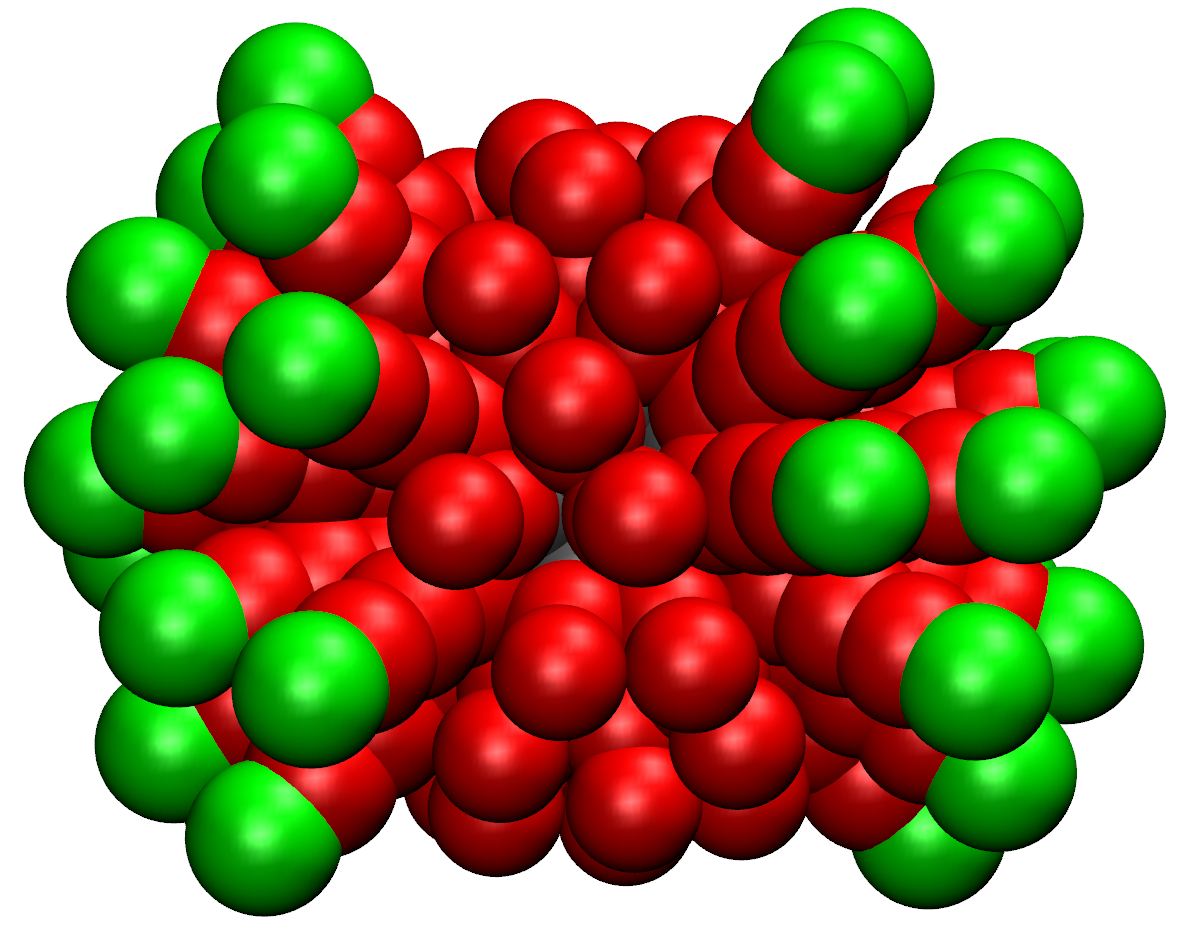
\includegraphics[width=0.25\textwidth]{./img/coatings/striped}%
	}\qquad\qquad%
	\subfloat[Random arranged \acs{NP}]{%
		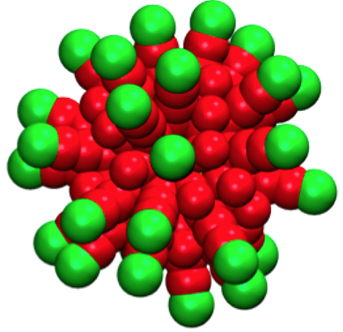
\includegraphics[width=0.25\textwidth]{./img/coatings/random11}%
	}\\%
	\subfloat[\acs{NP} in hydrophobic contact]{%
		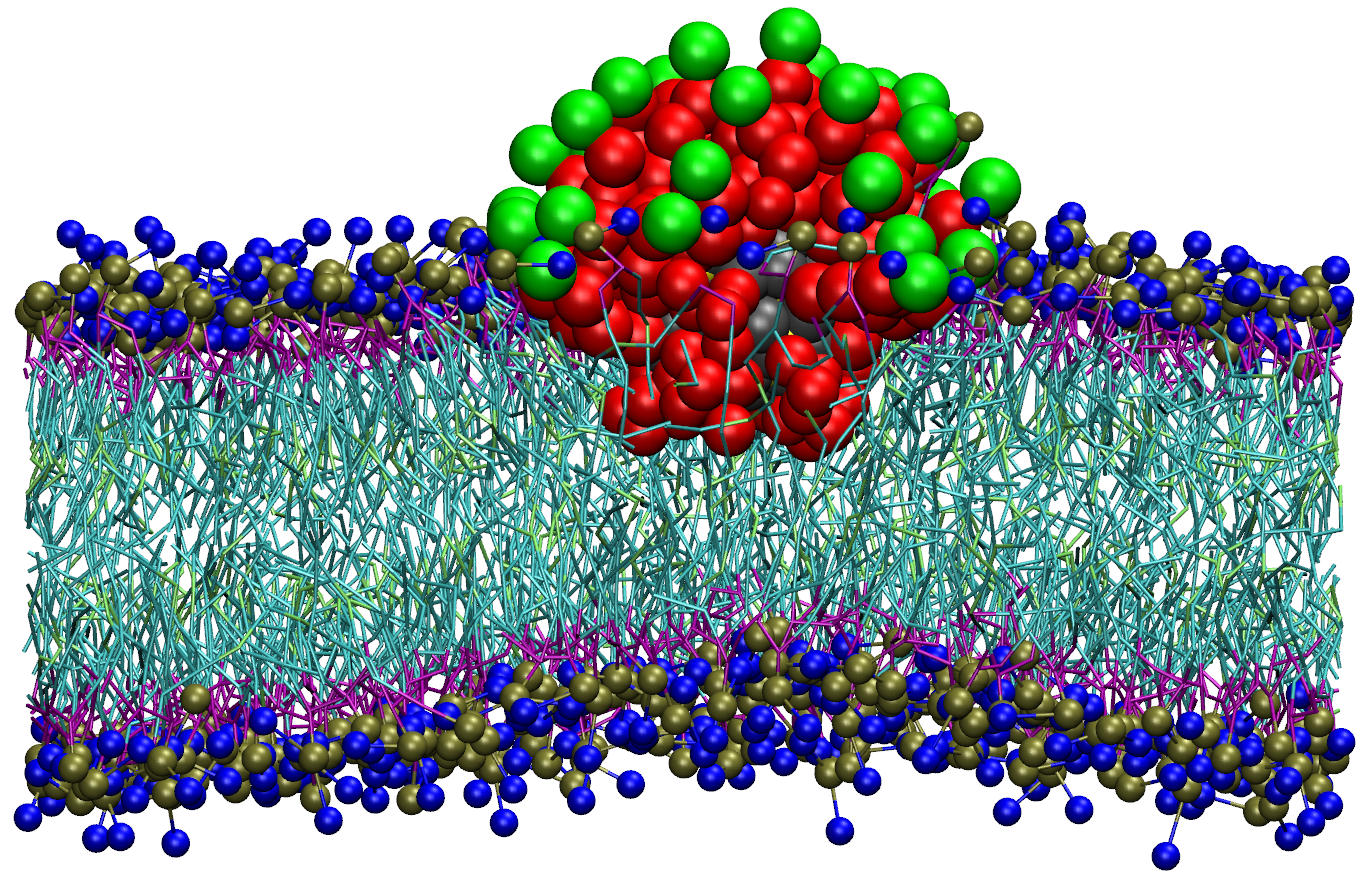
\includegraphics[width=0.7\textwidth]{./img/NPMembrane}%
	}%
	\caption{(a) The striped arranged \acs{NP}. (b) The random arranged \acs{NP}. (c) Striped \acs{NP} interacting with the model lipid membrane. In red the hydrophobic beads and in green the negatively charged beads of the \acs{NP} ligands. In gray the sulfur atoms of the \acs{NP}'s core. In blue the choline groups, in tan the phosphate groups and in violet the glycerol groups of the lipid heads. The lipid tails are shown as cyan colored stick. Beads of the water solvent are not shown for clarity.}
	\label{fig:NPSummary}
\end{figure}

In particular, I focused on the interaction between monolayer--protected, anionic \ac{AuNP} and model lipid bilayers. The surface charge of the ligand--protected \ac{NP}s makes them water--soluble, but it also affects their interaction with lipid membranes. Our simulations aimed at clarifying the role played by electrostatic during the passive \ac{NP}--membrane interaction. In particular, we have performed unbiased \ac{MD} simulations and free energy calculations using models that differ in resolution and in the way they treat electrostatic interactions. We compared the outcomes of the different models with respect to a. the energetics of the \ac{NP}--membranes interactions and b. the molecular mechanisms involved.

In the following, we summarize the main results and the future perspectives.


%This thesis is focused on study the role played by the electrostatic interaction and the different levels of accuracy of its treatment in the one anchor process --- from the \ac{NP} in the hydrophobic state to the state in which one charged \ac{MUS} ligand is anchored to the opposite leaflet --- an important stage in the anionic, passivated \ac{AuNP} interaction with biological membrane. We used computational methods, \ac{MD} with a popular \ac{CG} \ac{FF} for biomolecular applications, the \martini \ac{FF} \cite{Martini}, to simulate the system and advanced sampling techniques, metadynamics \cite{MetadParrinello}, to perform free energy calculations: speed--up the anchoring process and try to estimate the free energy profile involved in the forward process, the anchoring, and the backward process, the dis--anchoring of the charged ligand terminal. The achieved results, with a more sophisticated \ac{CG} model, allow us also to investigate the membrane deformation and the molecular processes involved in the charged ligand translocation, such as the leaflets deformation due to the dragging effect of water and lipid heads by the charged ligand terminal. In the following, we summarize the main achieved results and the future perspectives.

% \begin{enumerate}[label=\roman*.]
% 	\item \textit{Free energy calculation.} With the comparison we made between different \ac{CG} models: the \ac{STD} \martini, \martini with \ac{PME} and \martini with both \ac{PME}$+$\ac{PW} and the atomistic one, we understand, at the contrary of what we thought, that \textit{the path way for the forward and backward processes are evidently different causing a sampling error in the whole \ac{FES} of the translocation process}. In particular, for the striped (\acs{MUS}:\acs{OT} $1$:$1$) \ac{NP} both the barriers are almost identically and equal to about $100$~kJ/mol; for the random (\acs{MUS}:\acs{OT} $1$:$1$) \ac{NP} the forward barrier is equal to about $60$~kJ/mol while the backward one is higher than the forward of about $35$~kJ/mol.\\
% \textit{The future perspectives} are related in more studies of such free energy profiles: trying to pull down other ligands if one is already present in the anchored state and understand if the translocation process is helped or hindered with other \acp{NP} on the lipid bilayer. We understand that the used \ac{CV} suffers of some issues that leads in systematic sampling errors due to the hidden energy barriers. Hence can be of interest trying to find another \ac{CV} or try to increase the dimensionality of it using more than one \acp{CV}: as example, we could use the number of contacts between the charged ligand terminal and the lipid or both the \acp{CV}. These attempts can also be useful in finding other molecular mechanism that make the translocation process favorable.
%
% 	\item Thanks to its extremely high computational efficiency, we believe that \textit{the \ac{STD}} \martini \textit{\ac{FF} remains indispensable for qualitatively results} and for understand the first molecular basis of a process, without all the computational issues related to a finer model. Unfortunately, \textit{it is insufficient for obtain quantitative results}, especially of such processes that strongly depends on the electrostatic interaction. Despite the slight worsening of the computational performance, we have to include the \ac{PME} method for a long--range treatment of the electrostatic interaction and the \ac{PW} model in order to cancel out the use of an implicit medium that change the behavior of an hydrophobic environment, such like the core of a lipid membrane, and to achieve a better behavior of the water solvent.%
%
% 	\item \textit{We have confirmed the trend between the striped and the random \acp{NP}}, as observed with the \ac{STD} \martini \ac{FF} in \cite{ourPaper}. The striped \ac{NP} presents a forward energy barrier higher than the random one of about $40$~kJ/mol. The future perspectives are related to investigate how the \ac{FES} change with a multicomponent lipid membrane, for example adding cholesterol, that increases the rigidity of the membrane; how the free energy profile change with different degrees of hydrophobicity of the \ac{NP}, using ligands with different length; different kind of ligands; different surface arrangements; or using larger \acp{NP} that allow to play with this different configurations of the ligands.%
% \end{enumerate}

\section{free energy calculation}
With advanced sampling techniques \textit{I estimated the free energy profiles of one charged ligand translocation across the lipid membrane}, as shown in figure~(\ref{fig:coglionazzo}), using \acp{NP} with different surface ligands arrangements and different models to treat the electrostatic interaction at \ac{CG} level. For the striped (\acs{MUS}:\acs{OT} $1$:$1$) \ac{NP} I have found that both the energy barriers are almost identically and equal to about $100$~kJ/mol; for the random (\acs{MUS}:\acs{OT} $1$:$1$) \ac{NP} the forward energy barrier is equal to about $60$~kJ/mol while the backward one is higher than the forward of about $35$~kJ/mol. Furthermore, thanks to the atomistic results --- courtesy of Federica Simonelli --- a comparison between the \ac{CG} models and the atomistic one has been made. From this, we understand that a better treatment of the electrostatic interaction is necessary to achieve results that are approaching the atomistic model, one of the most real model achievable in a classical \ac{MD} simulation.

\begin{figure}[ht]
	\center
	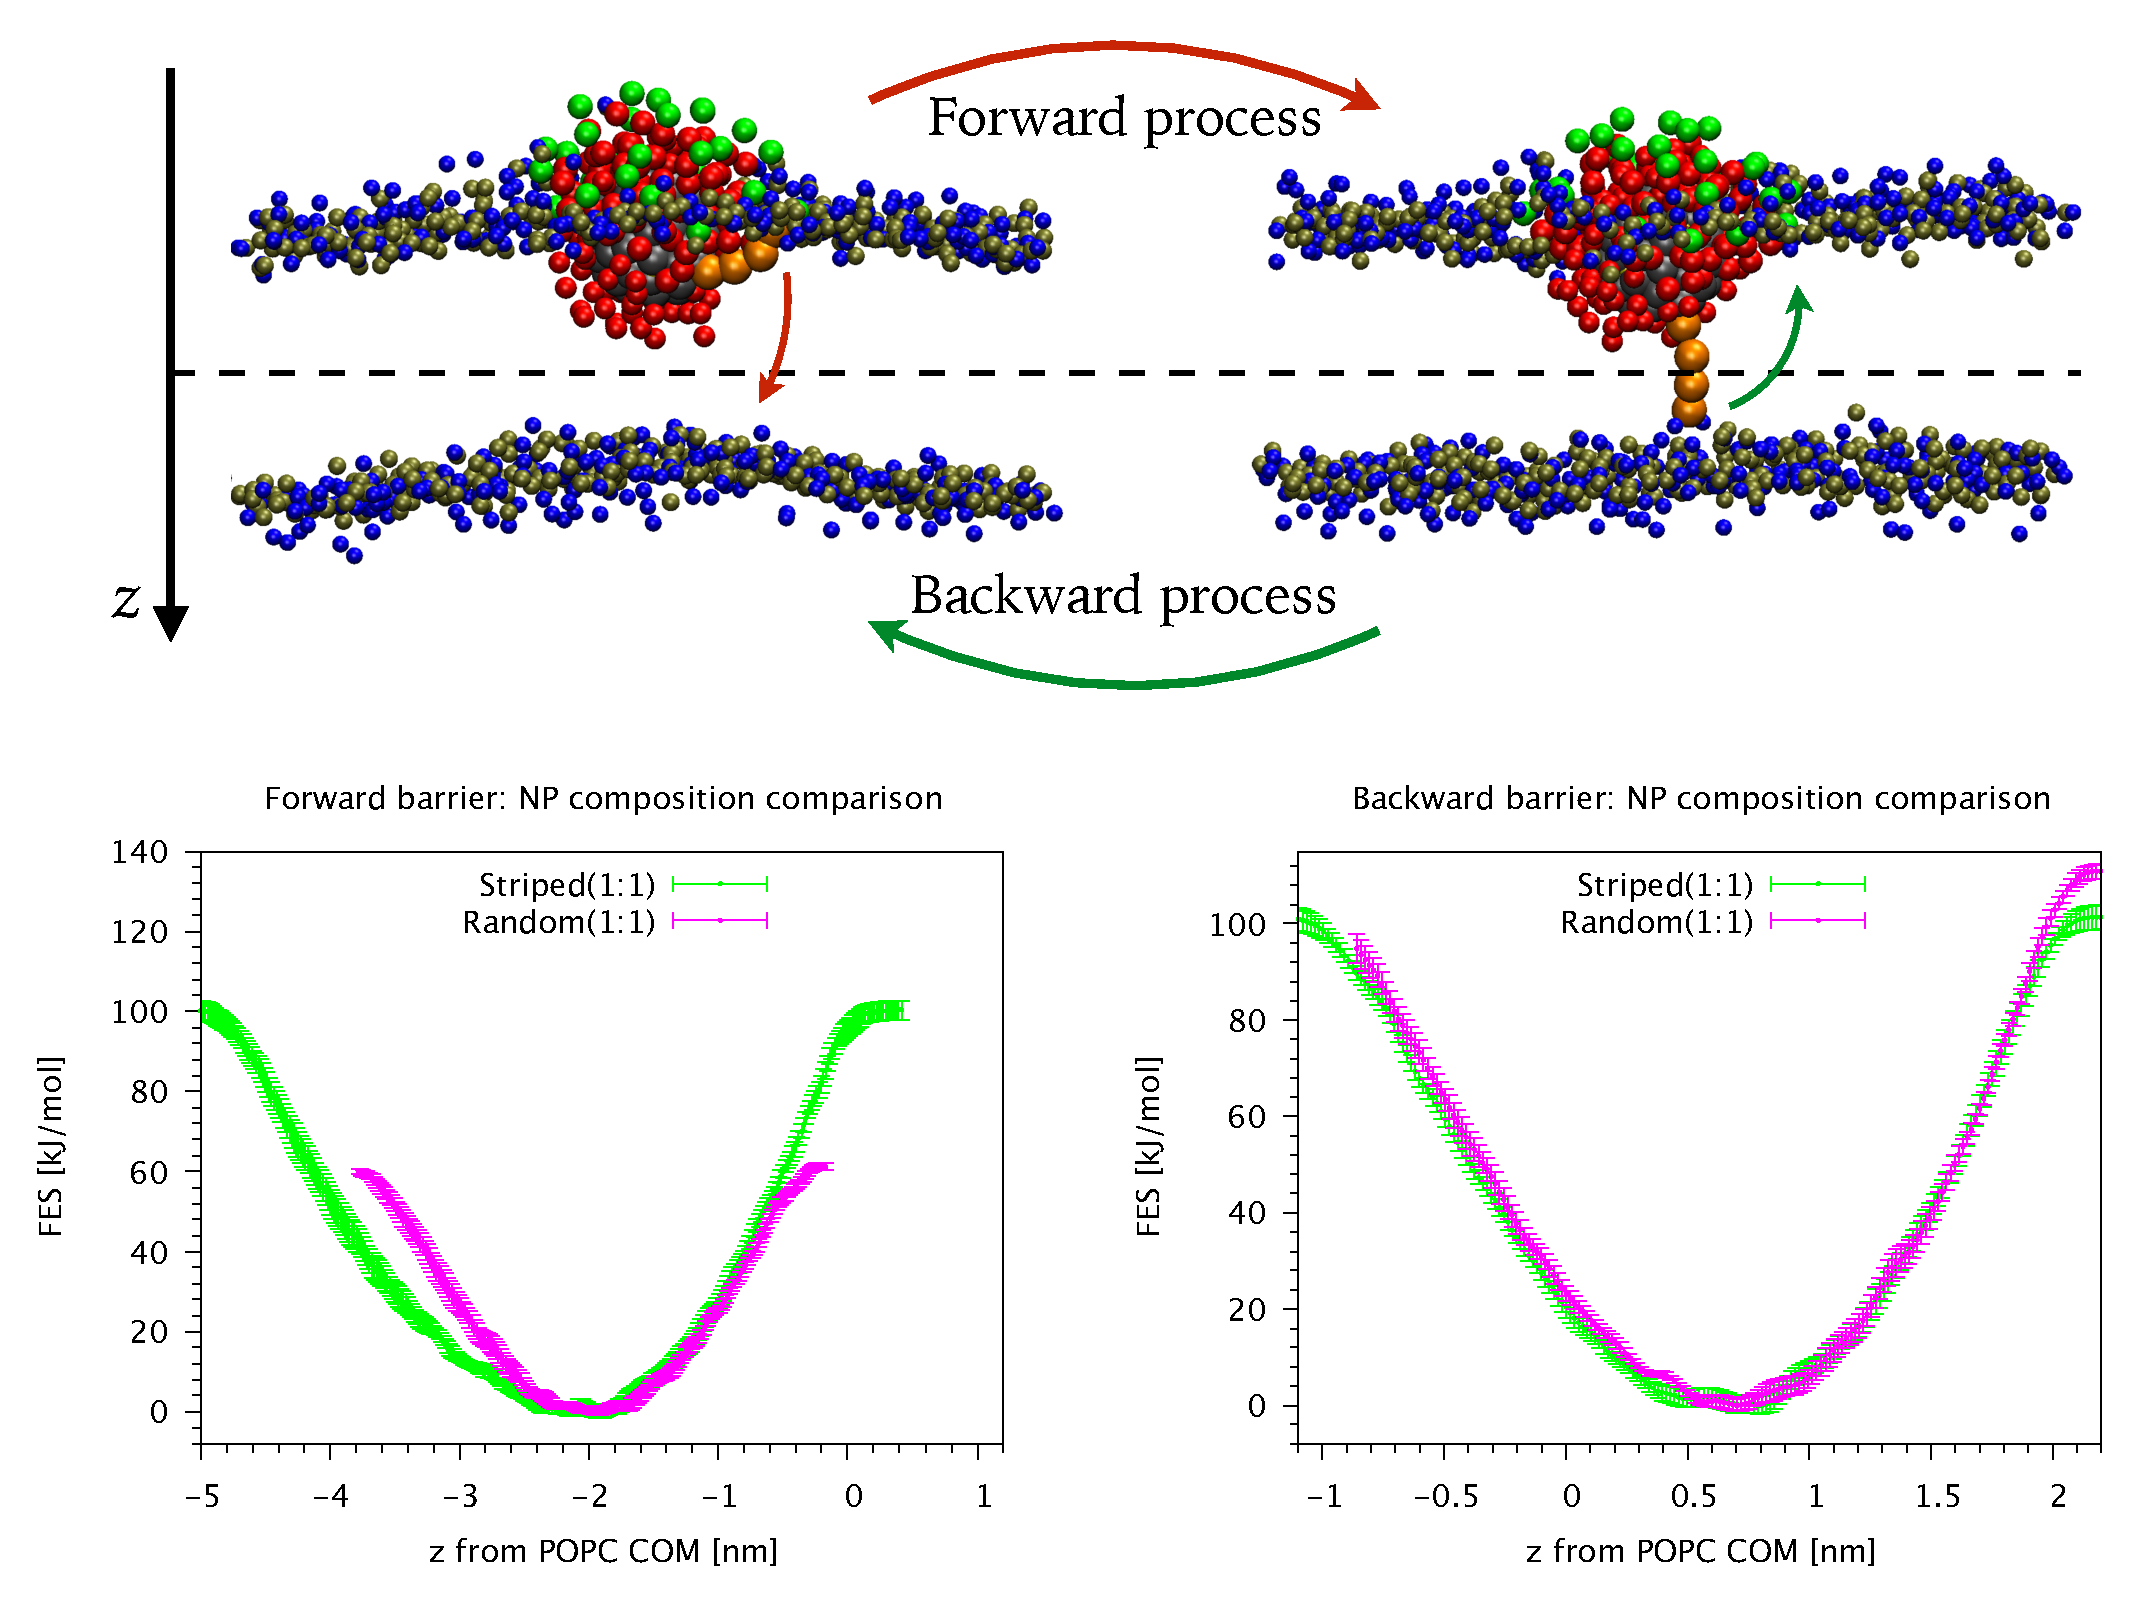
\includegraphics[width=\textwidth]{./img/coglionazzo}
	\caption{Top: a charged ligand (orange beads) during the membrane translocation process: from the hydrophobic contact in the entrance leaflet to one anchor state in the opposite leaflet, forward process; and \textit{vice versa}, backward process. The dashed line is the \acs{COM} of the bilayer. Color code as in figure~(\ref{fig:NPSummary}). Water beads and lipid tails are not shown. Bottom: the related free energy profiles, separately for the forward (left panel) and the backward process (right panel), for the striped (green) and the random (violet) \acp{NP}. }
	\label{fig:coglionazzo}
\end{figure}

\textit{The future perspectives} are related in more studies of these free energy profiles. In particular, how the free energy profiles of the translocation process depends on the number of ligands already anchored in the anchoring leaflet and if it is helped or hindered with other \acp{NP} embedded in the lipid bilayer. The used \ac{CV} suffers of some issues that leads in systematic sampling errors due to the hidden energy barriers. Hence can be of interest trying to find other \acp{CV}: as example, we could use also the number of contacts between the charged ligand terminal and the lipid. These attempts can also be useful in finding other molecular mechanism that make the translocation process more favorable.

\section{coarse--grained models}
Thanks to its extremely high computational efficiency, we believe that \textit{the \ac{STD}} \martini \textit{\ac{CG} \ac{FF} remains indispensable for qualitatively results} and for understand the first molecular mechanism of a process, without all the computational issues related to a finer model. Unfortunately, \textit{it is insufficient for obtain quantitative results}, especially of such processes that strongly depends on the electrostatic interaction. Despite the decrease of the computational performance, we have to include the \ac{PME} method for a long--range treatment of the electrostatic interaction and a better \ac{CG} water model in order increase the behavior of the water solvent but also the hydrophobic regions of the system, ex. the hydrophobic core of a lipid bilayer. 

\section{surface arrangements}
\textit{We have confirmed that the surface arrangements of the \ac{NP} ligands can affect the free energy profiles} involved in the \ac{NP}--membrane interactions, as what is observed with the \ac{STD} \martini \ac{FF} in \cite{ourPaper}. The striped \ac{NP} presents a forward energy barrier higher than the random one of about $40$~kJ/mol. 

\textit{The future perspectives} are related to investigate how the free energy profile is affected by a multicomponent lipid membrane, for example adding cholesterol, that increases the rigidity of the membrane. How the free energy profile change with different degrees of hydrophobicity of the \acp{NP}; or using ligands with different length or different kind of ligands; different surface arrangements; or using larger \acp{NP} that allow to play with this different configurations.


%restore toc configuration
\restoretoc
\endgroup